\documentclass{beamer}
\beamertemplatenavigationsymbolsempty{}
\usetheme{Goettingen}
\setbeamertemplate{footline}[frame number]
\usecolortheme{sidebartab}

%\setbeameroption{show only notes} % Only notes
%\setbeameroption{show notes on second screen=right} % Both

\mode<presentation>
\title[WebSocket]{Performance Evaluation of WebSocket Protocol for Implementation of Full-Duplex Web Streams}
\author{Oleg Bilovus}
\institute{Università degli Studi di Salerno}
\date[SRF 1st]{1st Scalability Research Forum}

\begin{document}
\begin{frame}
    \titlepage{}
    \note{We will talk about WebSockets and compare its performance with TCP Socket. But, before divinng into analysing the performance we need to understand why we needed WebSockets and whats they are.}
\end{frame}

\AtBeginSection[]{ \begin{frame}\frametitle{Outline} \tableofcontents[currentsection]\end{frame} }

\section{Background}
\begin{frame}
    \frametitle{Background}
    \begin{itemize}[<+->]
        \item \emph{Historically}, creating \alert<+->{web applications} that need \alert<+->{bidirectional
                  communication} between a \alert<+->{client} and a \alert<+->{server} has required an \alert<+->{abuse of
                  HTTP to poll} the server for updates while sending upstream notifications as
              \alert<+->{distinct HTTP calls}.
              \note{bidirectional means the server and the client can send data to each other at any time}
    \end{itemize}
\end{frame}

\subsection{HTTP polling}
\begin{frame}
    \frametitle{HTTP polling}
    Check whether the server is changed in a while, thereby performing incremental updates.
    \begin{columns}
        \begin{column}{0.7\textwidth}
            \begin{figure}
                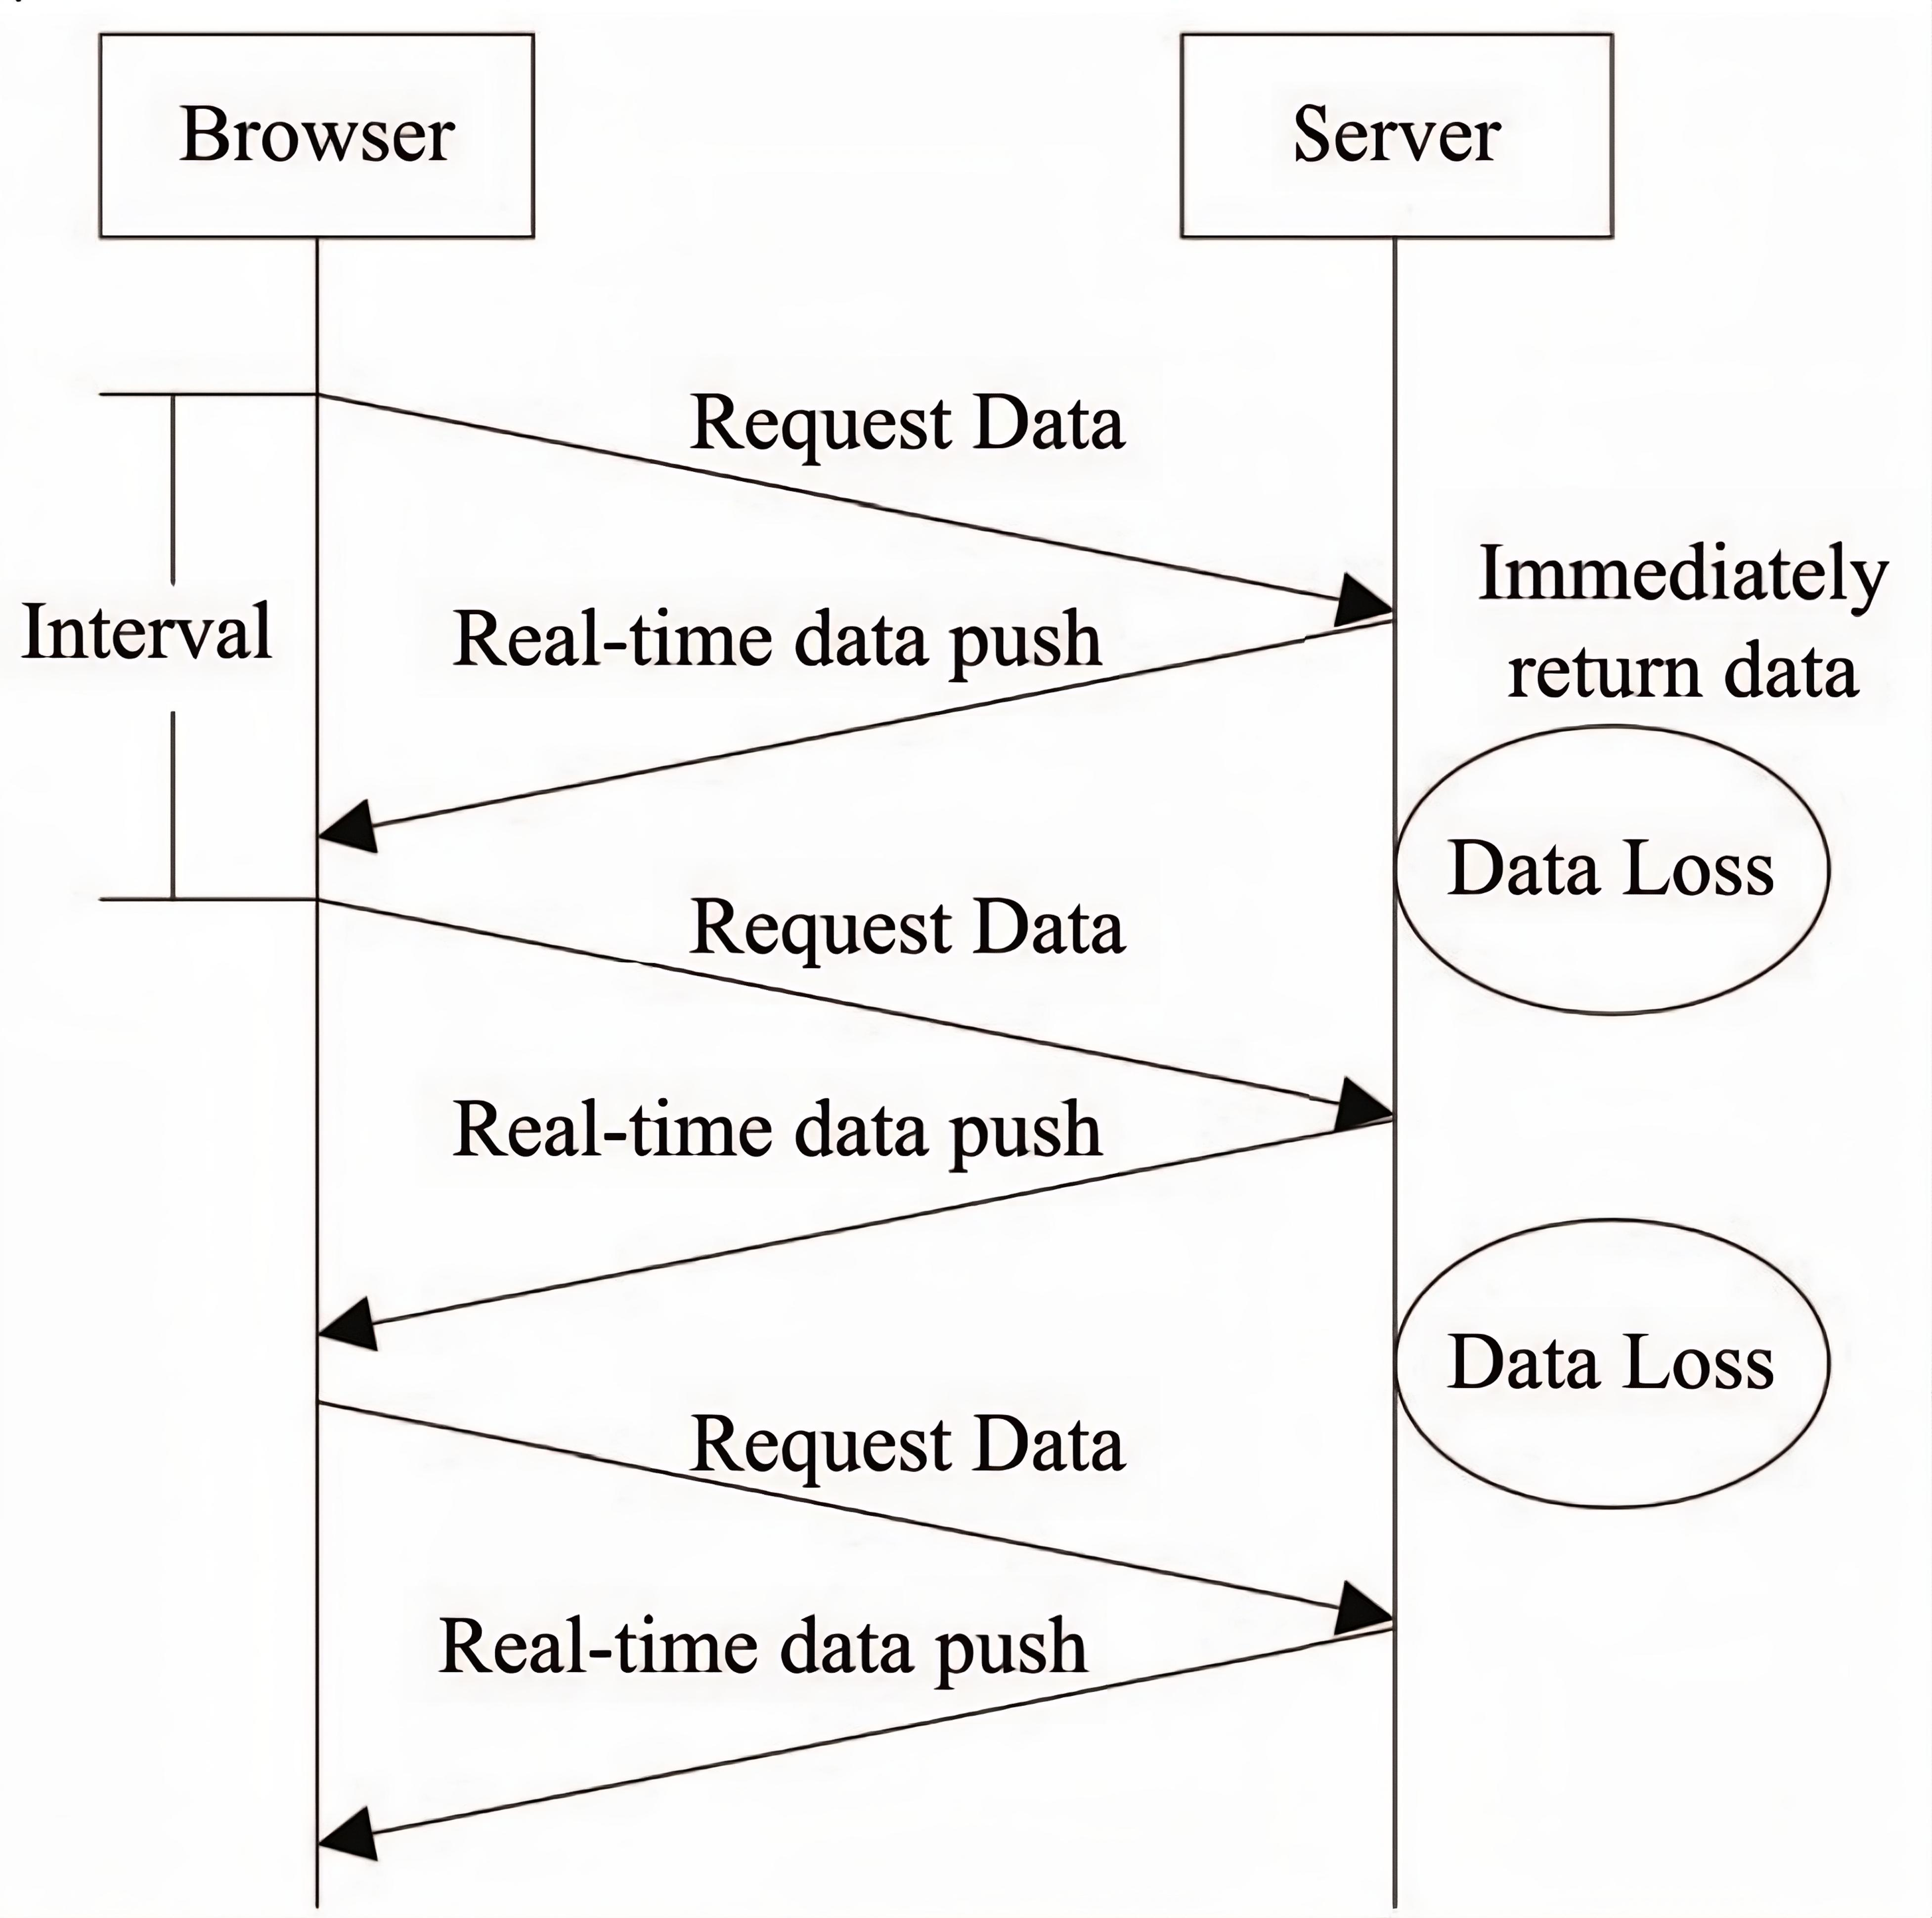
\includegraphics[width=0.7\textwidth]{images/polling.jpeg}
            \end{figure}
        \end{column}
        \begin{column}<+->{0.35\textwidth}
            \begin{itemize}[<+->]
                \item How often to query?
                \item Continuously \alert{short interval} requests will be \alert{washed away} the
                      server. \note{A client can send data and ask for data at the same time. But, if
                          client has no data and server has no data, a request and response will still be
                          generated with all the HTTP headers and thus wasting resources.}
                \item \alert{Long interval} will require more time to reach the client, \alert{no real-time} data.
                      \note{no real-time data because while the client waits, an event could occur and the client will know about it only when the timeout expires.}
            \end{itemize}
        \end{column}
    \end{columns}
\end{frame}

\subsection{HTTP long polling}
\begin{frame}
    \frametitle{HTTP long polling}
    When a client sends a data request, the server will block the request until there is data transfer or timeout before returning.
    \begin{columns}
        \begin{column}{0.7\textwidth}
            \begin{figure}
                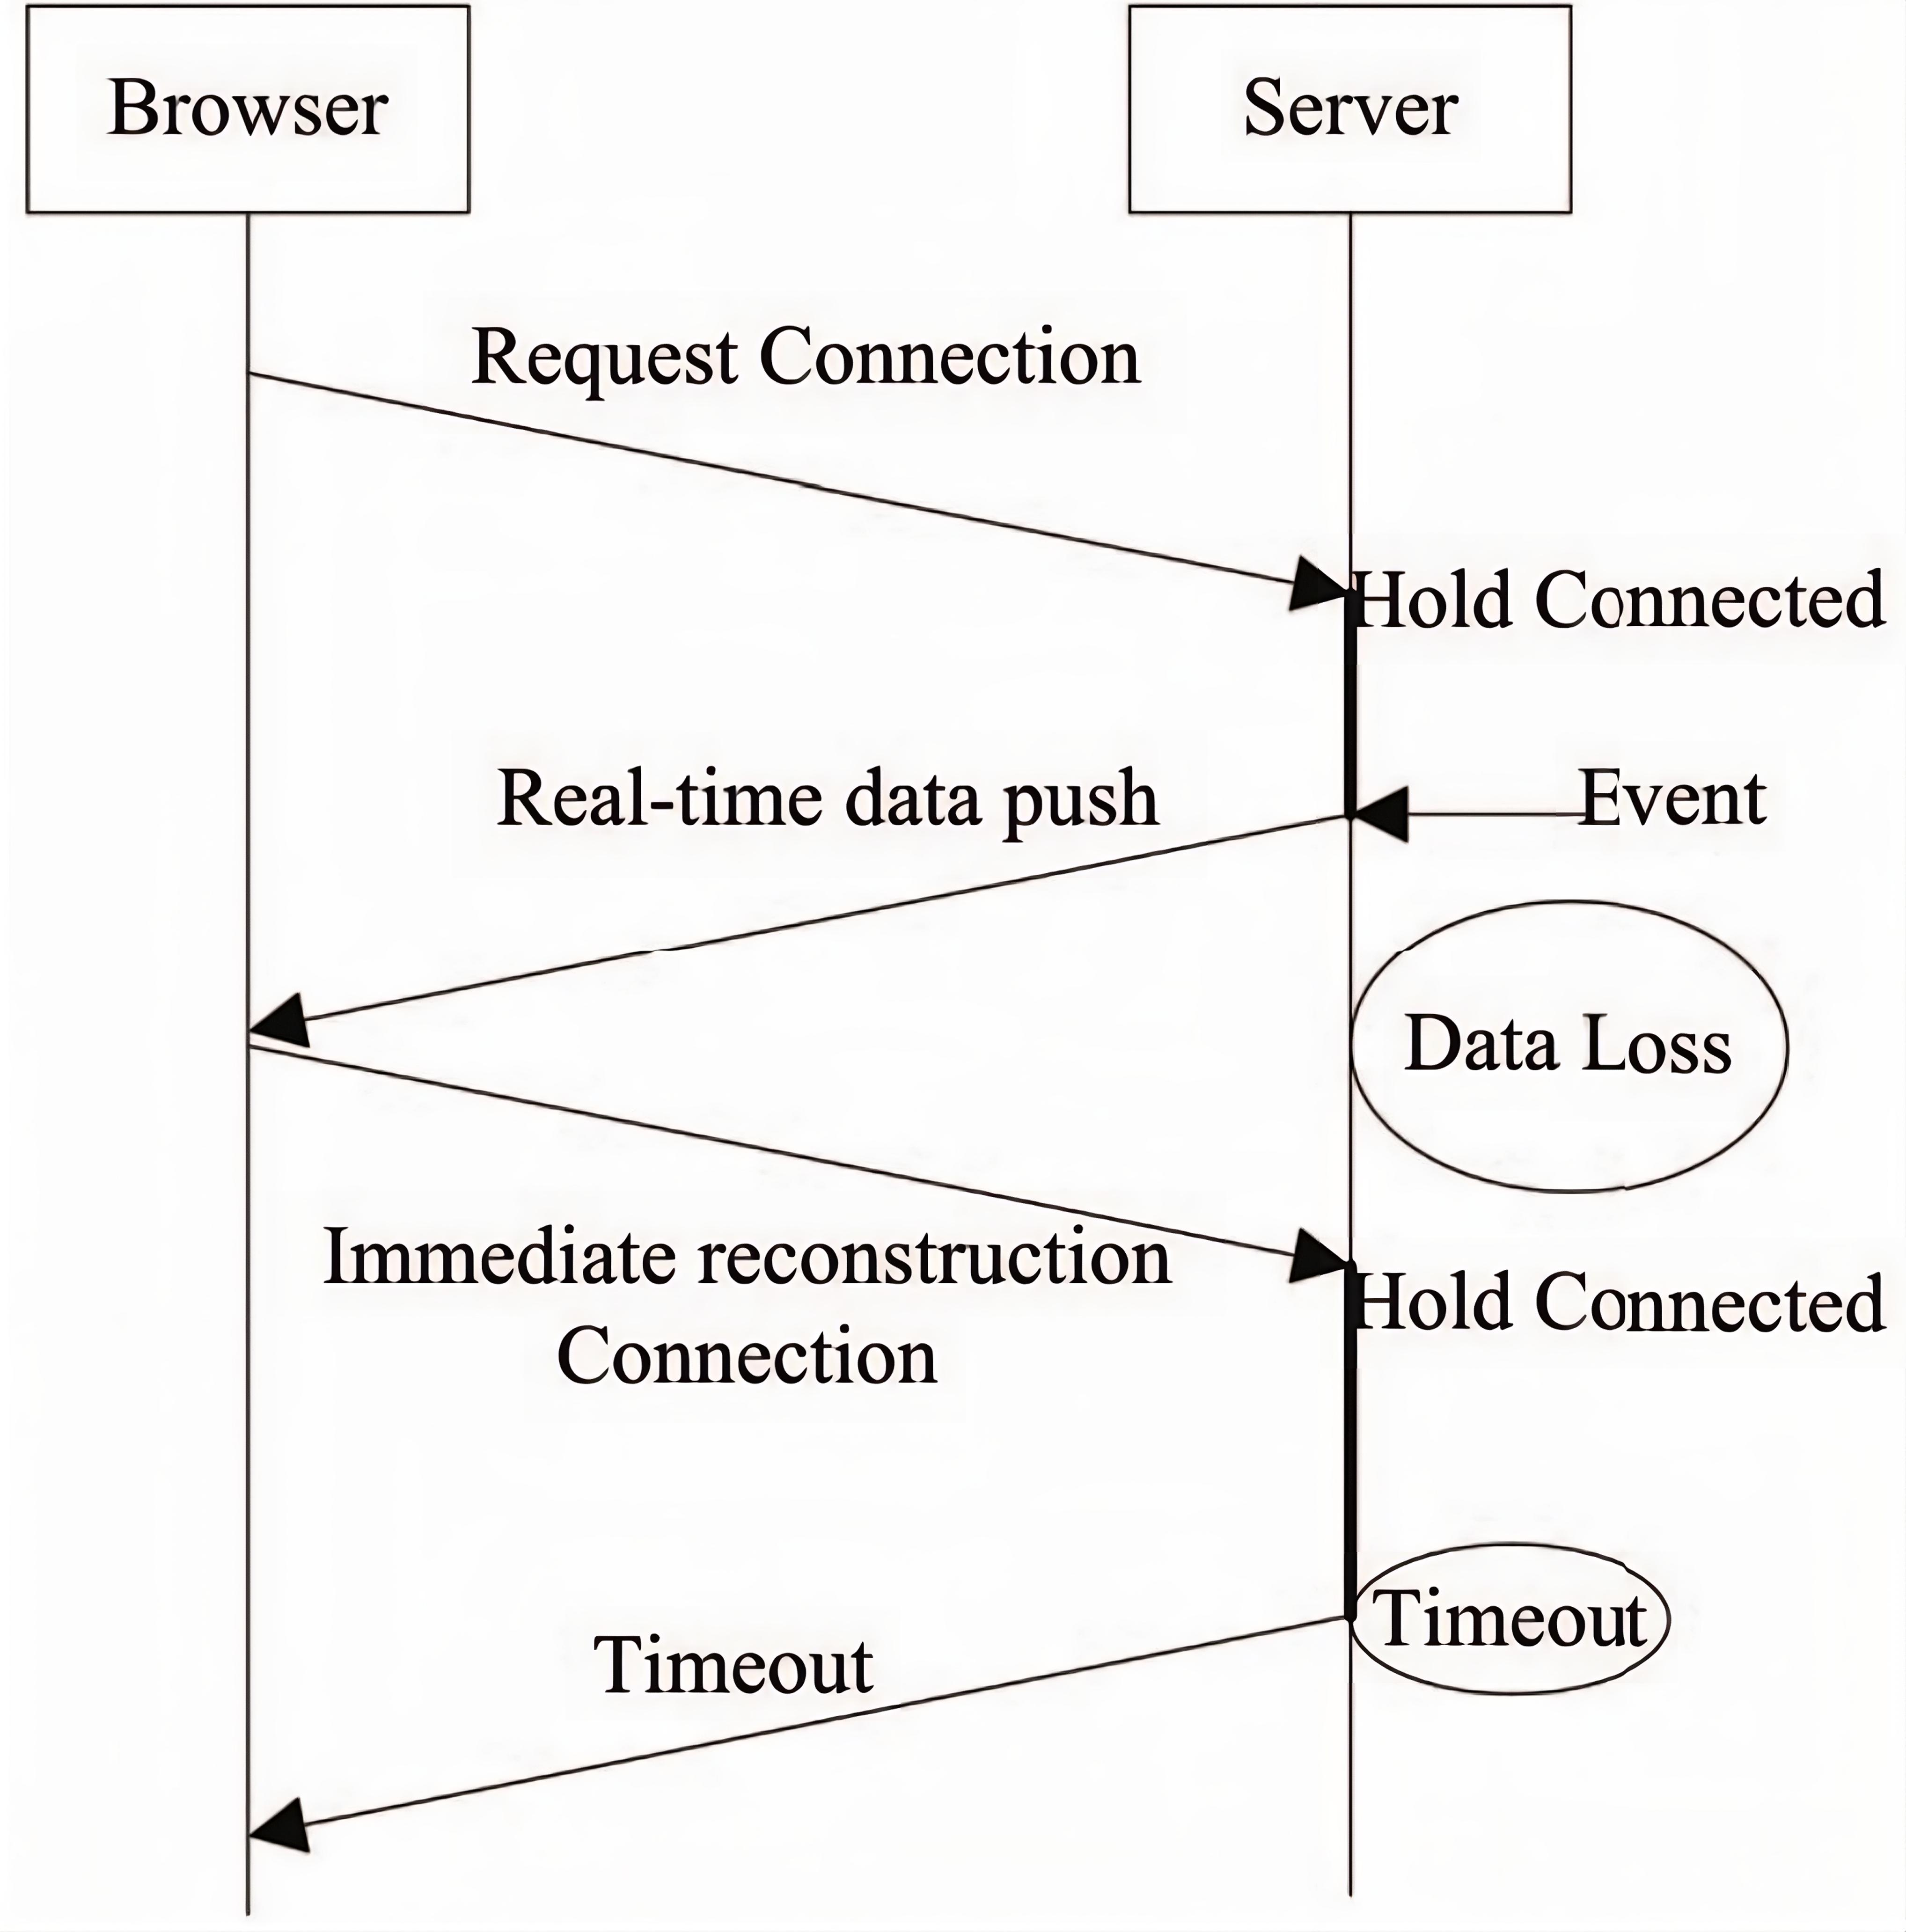
\includegraphics[width=0.7\textwidth]{images/long_polling.jpeg}
            \end{figure}
            \note{Can hold the connection up to a certain time, after that a timeout is execed and need a new connection.}
        \end{column}
        \begin{column}<+->{0.35\textwidth}
            \begin{itemize}[<+->]
                \item {\color{green} Solve the short polling frequency to access the server.}
                \item \alert{No bidirectional communication}, server push data.
                      \note{No biderectional because the client may only send data the first time but then it will only receive until a timeout and another request is made.}
                      \note{In the normal polling we could have biderectional because the interval was shorter.}
            \end{itemize}
        \end{column}
    \end{columns}
\end{frame}

\subsection{Streaming}
\begin{frame}
    \frametitle{Streaming}
    Iframe embed a hidden frame in an HTML page, then set it as a long connection request, thus the server can send data to the clients constantly.
    \note{iframe is an html page inside another.}
    \begin{columns}
        \begin{column}{0.7\textwidth}
            \begin{figure}
                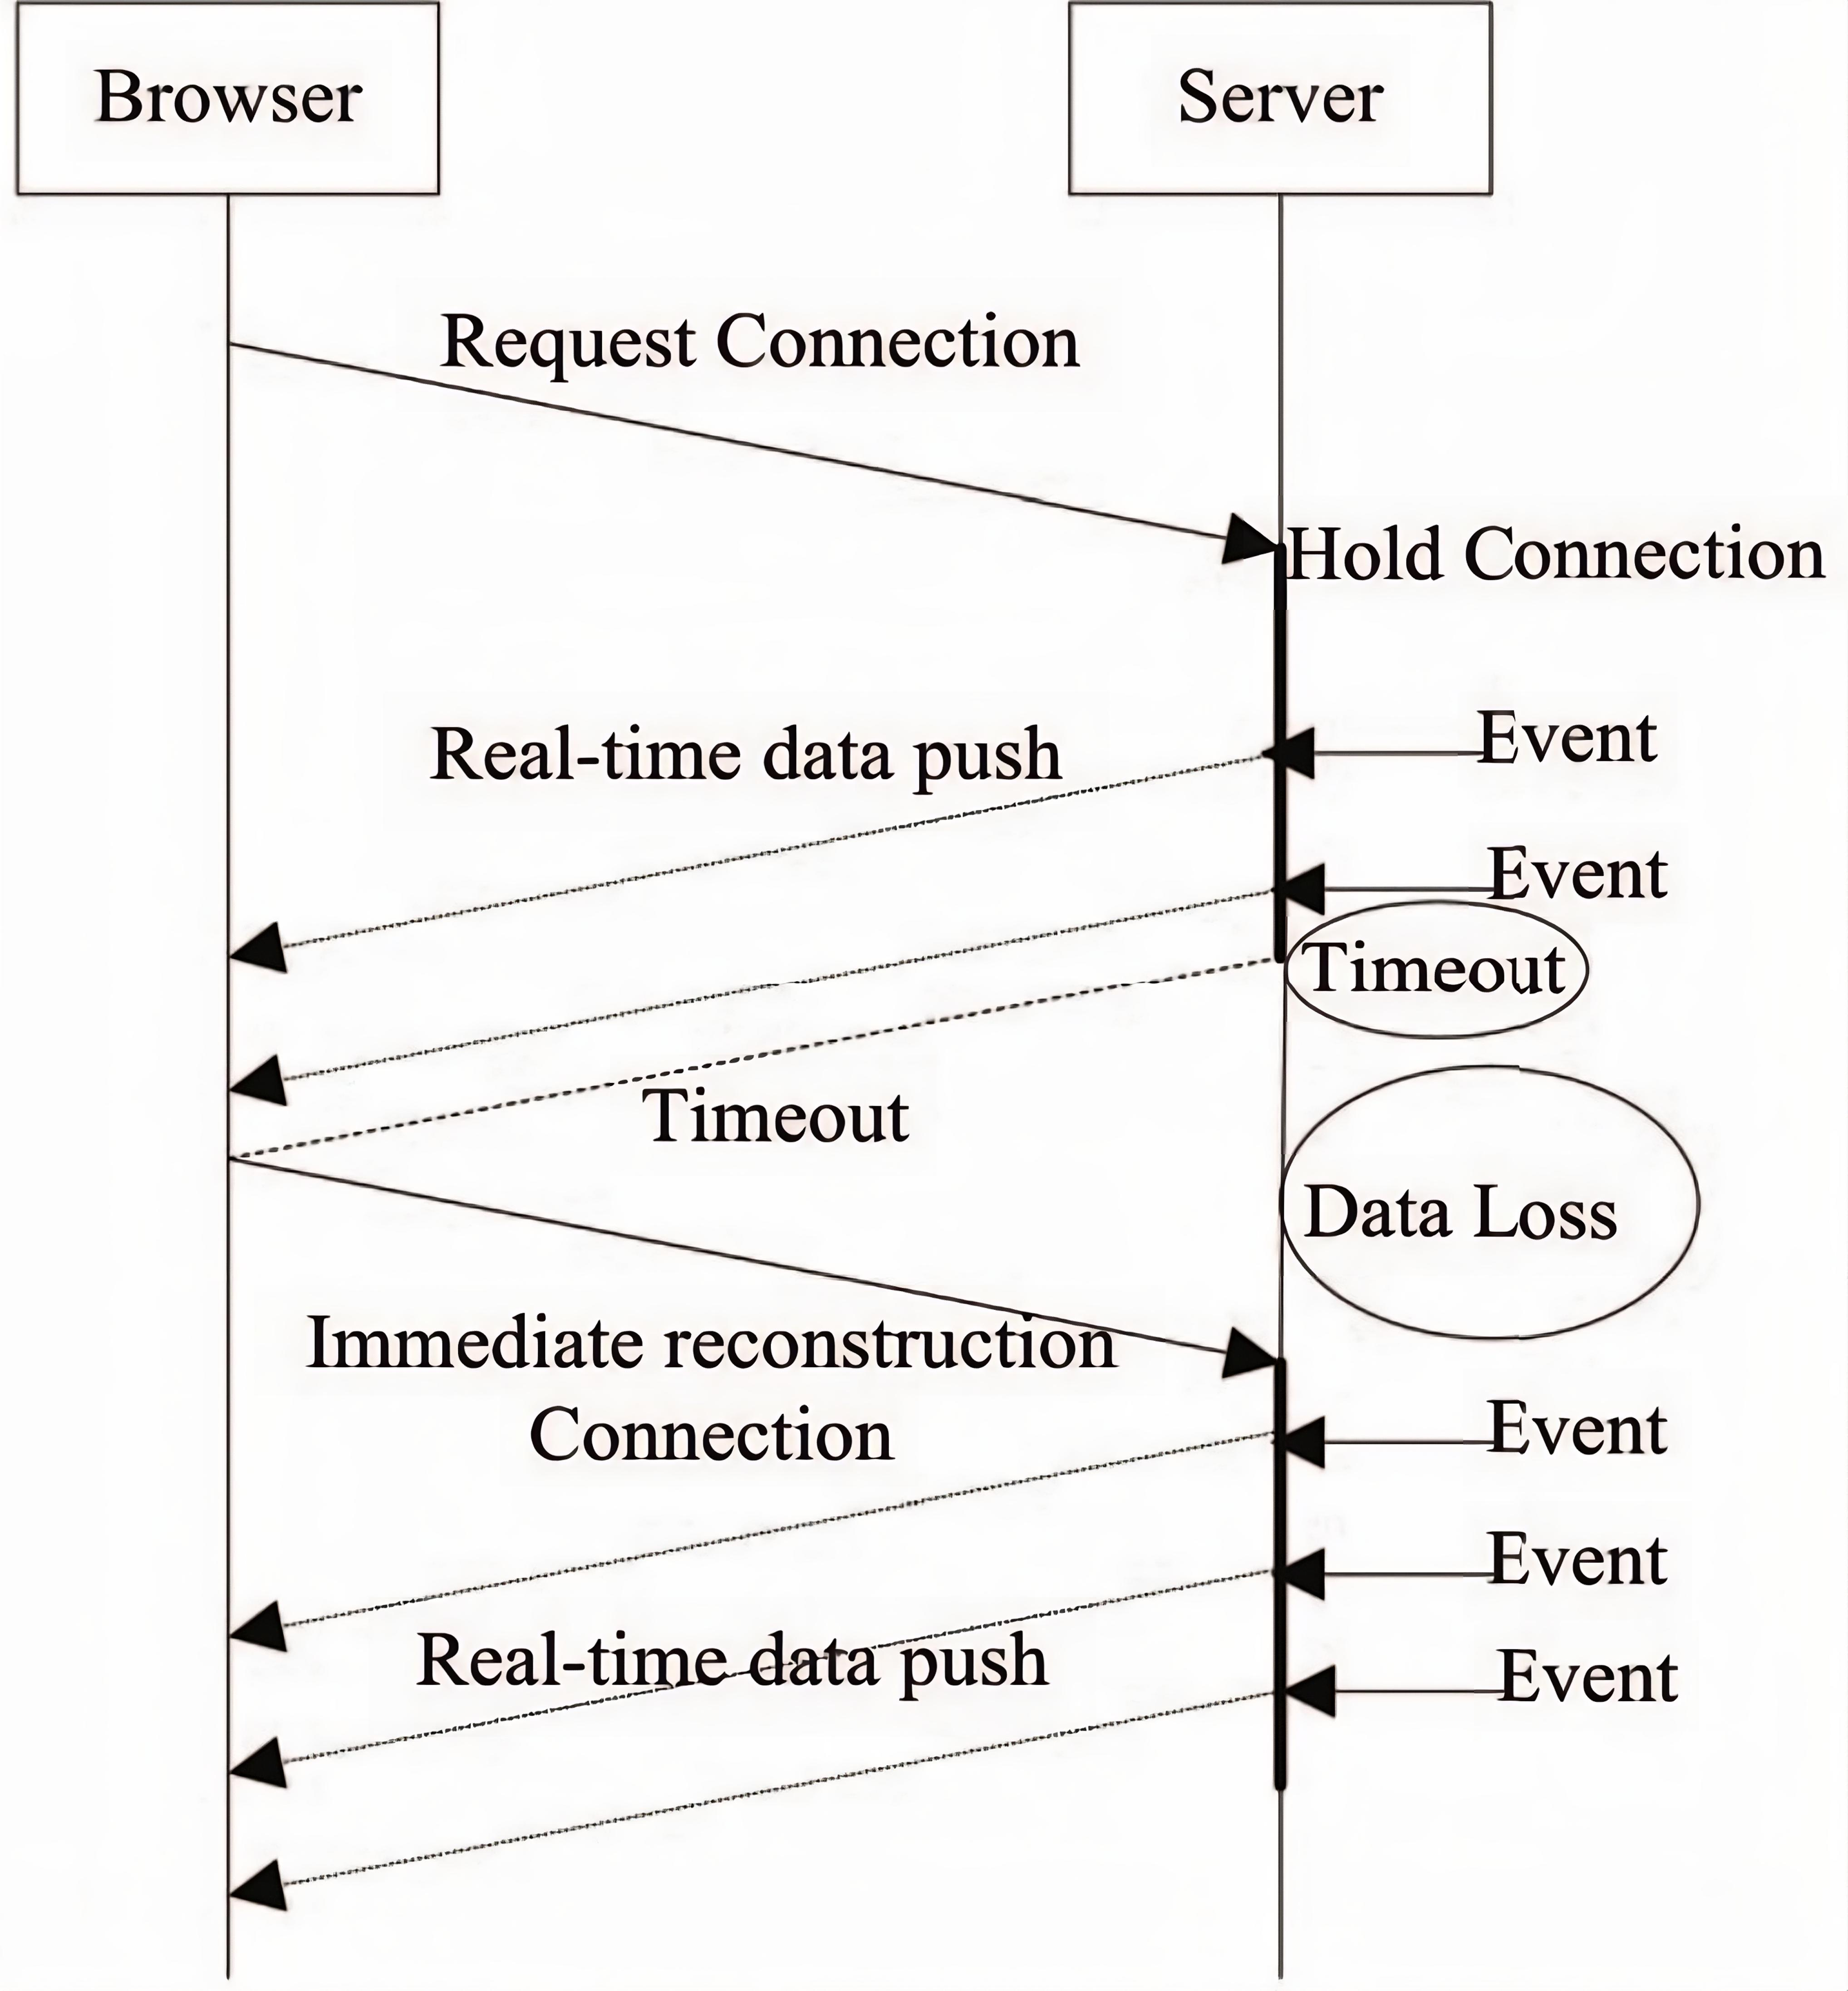
\includegraphics[width=0.7\textwidth]{images/streaming.jpeg}
            \end{figure}
        \end{column}
        \begin{column}<+->{0.35\textwidth}
            \begin{itemize}[<+->]
                \item It can sends {\color{green} multiple events} from a {\color{green} single
                              request}.
                \item But, it increase the \alert{burden on the server}, causing the server
                      \alert{performance degradation}, or even collapse. \note{Because the server
                          need to keep the connections alive.}
                \item \alert{No bidirectional communication.}
            \end{itemize}
        \end{column}
    \end{columns}
\end{frame}

\section{WebSocket protocol}

\subsection{Definition}
\begin{frame}
    \frametitle{RFC 6455}
    \framesubtitle{Keywords}
    \begin{itemize}[<+->]
        \item The WebSocket Protocol enables \alert<+->{two-way communication} between a
              \alert<+->{client} running untrusted code in a controlled environment to a
              \alert<+->{remote host} that has \alert<+->{opted-in} to communications from
              that code. \note{opted-in is important because with polling any HTTP server
                  would accept it, but here additional steps are needed.}
        \item The protocol consists of an opening \alert<+->{handshake} followed by basic
              \alert<+->{message framing}, layered over \alert<+->{TCP}. \note{handshake
                  means client and server have to agree that they can both use the protocol and
                  the server has to prove it.} \note{message framing because we do not want to
                  send every time the headers.} \note{TCP means it is reliable, no messages will
                  be lost.}
        \item The goal of this technology is to provide a mechanism for
              \alert<+->{browser-based} applications that need two-way communication with
              servers.
    \end{itemize}
\end{frame}

\subsection{Handshake}
\begin{frame}
    \frametitle{Handshake}
\end{frame}

\end{document}